% Start slide
\begin{frame}{}
    \vspace{2cm}
      \centering
      {\LARGE \textbf{Field of View and Obstacle Avoidance}\par}
      \vspace{2cm}
    \end{frame}
    
    
    \begin{frame}{Problem Formulation}
    \textbf{\large Input:}
    
    \begin{itemize}
      \item[-] racetrack (list of points and distances to boundaries)
      \item[-] list of circle obstacles
      \item[-] length $l$ and width $w$ of the vehicle (m)
      \item[-] coordinates of the view point (center of the vehicle)
      \item[-] vector of the view direction ($\vec{d_v}$)
      \item[-] maximal view distance $d$ (m)
      \item[-] maximal view angle $\alpha$ (rad)
    \end{itemize}
    \vspace{0.5cm}
    
    \begin{wrapfigure}{r}{0.42\textwidth}
      \vspace{-2.9cm}
      \begin{center}
        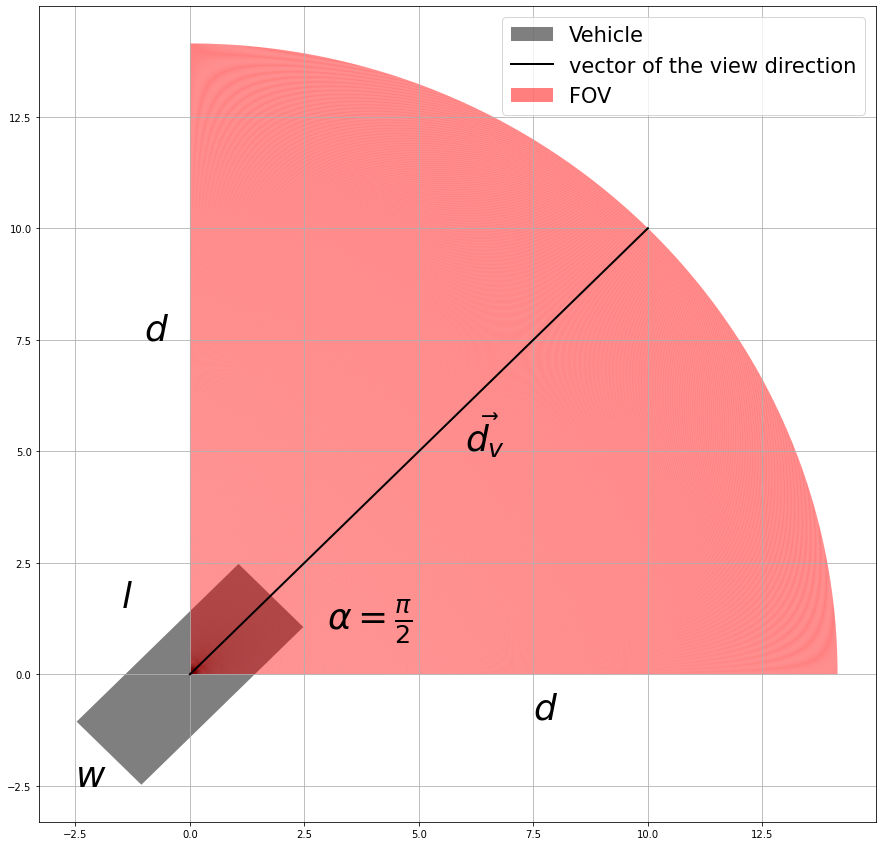
\includegraphics[width=0.42\textwidth]{final_pre_slides/root/fig_vasenkov/vehicle-params.jpg}
      \end{center}
    \end{wrapfigure}
    
    \textbf{\large Output:}
    \begin{itemize}
      \item[-] boundaries of the feasible gap
      \item[-] line for braking maneuver
    \end{itemize}
    
    \end{frame}
    
    % Method 1
    \begin{frame}{Problem solution: Splitting Vectors}
    % \vspace{-3.5cm}
    \textbf{\large Idea 1:}
    \begin{itemize}
      \item split the whole FOV with $K \geq 2$ vectors of length $d$ and find  points of intersection with boundaries and obstacles for all vectors (example with $K = 20$)
    \end{itemize}
    \begin{figure}
        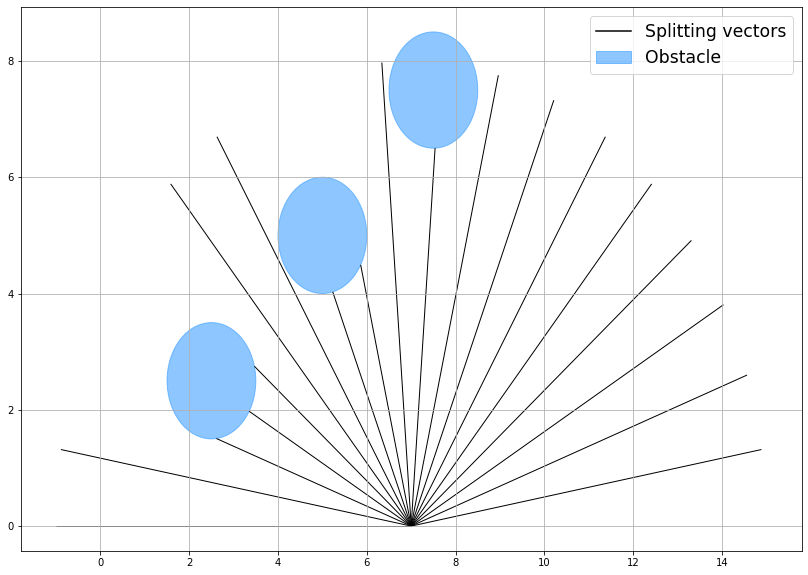
\includegraphics[width=0.8\linewidth]{final_pre_slides/root/fig_vasenkov/vs-demo.jpg}
        \label{fig:enter-label}
    \end{figure}
    \end{frame}
    
    \begin{frame}{Problem solution: Splitting Vectors}
    \textbf{\large Intersection with obstacle:}
    \begin{itemize}
      \item Equation of a Circle: $(x - x_c)^2 + (y - y_c)^2 = R^2$
      \item Equation of a Line: $x = x_0 + t(x_1 - x_0), y = y_0 + t(y_1 - y_0)$
      \item Solution: $t_{1,2} = \frac{-b \pm \sqrt{b^2 - 4ac}}{2a}$, where
      \item \begin{itemize}
          \item $a = (x_1 - x_0)^2 + (y_1 - y_0)^2$, assume $a \neq 0$
          
          \vspace{0.1cm}
          \item $b = 2(x_0 - x_c)(x_1 - x_0) + 2(y_0 - y_c)(y_1 - y_0)$
          
          \vspace{0.1cm}
          \item $c = (x_0 - x_c)^2 + (y_0 - y_c)^2 - R^2$ 
      \end{itemize}
    \end{itemize}
    \vspace{0.5cm}
    
    \begin{wrapfigure}{r}{0.55\textwidth}
      \vspace{-1.4cm}
      % \hspace{1.25cm}
      \begin{center}
        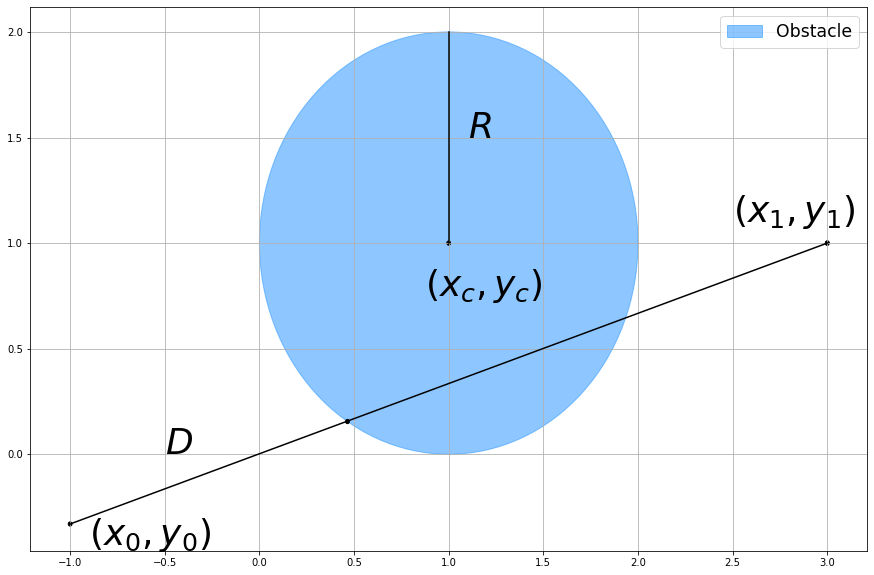
\includegraphics[width=0.55\textwidth]{final_pre_slides/root/fig_vasenkov/circle.jpg}
      \end{center}
    \end{wrapfigure}
    
    \textbf{\large No intersection if:}
    \begin{itemize}
        \item[-] $b^2-4ac < 0$, or
        \item[-] $||\vec{v_k}|| < D$, or
        \item[-] $t_i < 0, i \in \set{1,2}$
    \end{itemize}
    \end{frame}
    
    \begin{frame}{Problem solution: Splitting Vectors}
    \textbf{\large Intersection with boundary (for a single segment):}
    \begin{itemize}
      \item Segment has coordinates $(x_2, y_2), (x_3, y_3)$
      \item Construct Line Equation using $ax + by + c = 0$
      \item For the segment: $(y_3 - y_2)(x - x_2) - (x_3 - x_2)(y - y_2) = 0$
      \item For the vector: $x = x_0 + t(x_1 - x_0), y = y_0 + t(y_1 - y_0)$
    
      \vspace{0.05cm}
      \item Find a Solution: $t = \frac{(x_0 - x_2)(y_3 - y_2) - (x_3 - x_2)(y_0 - y_2)}{(x_3 - x_2)(y_1 - y_0) - (x_1 - x_0)(y_3 - y_2)}$
    \end{itemize}
    \vspace{0.25cm}
    \textbf{\large No intersection if:}
    \begin{itemize}
        \item[-] $t < 0$ or $t > 1$, or
        \item[-] $(x_3 - x_2)(y_1 - y_0) - (x_1 - x_0)(y_3 - y_2) = 0$
        \item[-] $x \notin [\min(x_2, x_3), \max(x_2, x_3)]$ or $y \notin [\min(y_2, y_3), \max(y_2, y_3)]$
    \end{itemize}
    
    \end{frame}
    
    \begin{frame}{Problem solution: Splitting Vectors}
    \textbf{\large Algorithm:}
    \begin{itemize}
      \item[-] $\vec{v_0} = \begin{bmatrix}
                                cos(\frac{\alpha}{2}) & sin(\frac{\alpha}{2}) \\
                                -sin(\frac{\alpha}{2}) & cos(\frac{\alpha}{2})
                            \end{bmatrix} \vec{d_v}$
            - find right bound vector
      \item[-] $\theta = \frac{\alpha}{K - 1}$ - find rotation step
      \item[-] $\vec{v_k} = \begin{bmatrix}
                                cos(\theta) & -sin(\theta) \\
                                sin(\theta) & cos(\theta)
                            \end{bmatrix}^k \vec{v_0}$ - find all splitting vectors
      \item[-] Iterate over all vectors $\vec{v_k}$, finding intersection with obstacles and boundaries
      \item[-] Find gap with maximal distance and sufficient width 
      \item[-] Output gap boundaries
    \end{itemize}
    \end{frame}
    
    % Method 2
    \begin{frame}{Problem solution: Tangent Lines}
    % \vspace{-3.5cm}
    \textbf{\large Idea 2:}
    \begin{itemize}
      \item split the whole FOV with tangent lines to all obstacles and boundaries, find feasible gap
    \end{itemize}
    \begin{figure}
        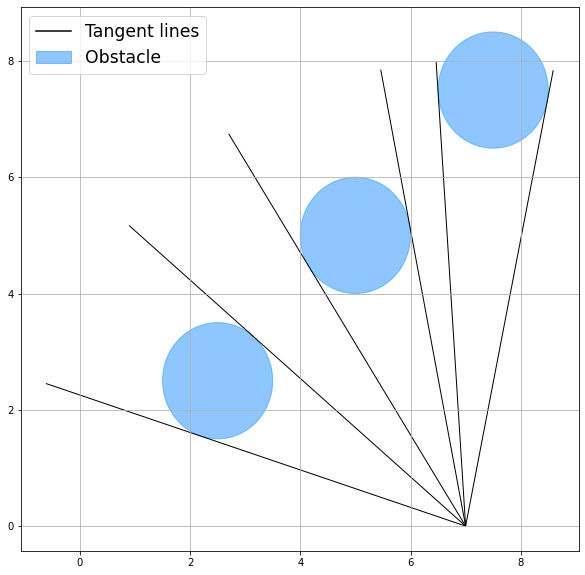
\includegraphics[width=0.65\linewidth]{final_pre_slides/root/fig_vasenkov/tangent-demo.jpg}
        \label{fig:enter-label}
    \end{figure}
    \end{frame}
    
    \begin{frame}{Problem solution: Tangent Lines}
    
    \vspace{-1cm}
    \textbf{\large Tangent Lines for a Circle Obstacle:}
    \begin{itemize}
      \item[-] Obtain direction vector $\vec{d_c} = (x_c - x_0, y_c - y_0)^T$
      \item[-] Rotate $\vec{d_c}$ by $\beta$ and $-\beta$ to obtain Tangent Lines direction vectors:
      \vspace{-0.45cm}
      \begin{center}
        \item $\vec{d_c^1}$ = \begin{bmatrix}
                                cos(\beta) & -sin(\beta) \\
                                sin(\beta) & cos(\beta)
                            \end{bmatrix} $\vec{d_c};$
              $\vec{d_c^2}$ = \begin{bmatrix}
                                cos(\beta) & sin(\beta) \\
                                -sin(\beta) & cos(\beta)
                            \end{bmatrix} $\vec{d_c}$
      \end{center}
    \end{itemize}
    
    \begin{wrapfigure}{r}{0.48\textwidth}
      \vspace{-1.5cm}
      \begin{center}
        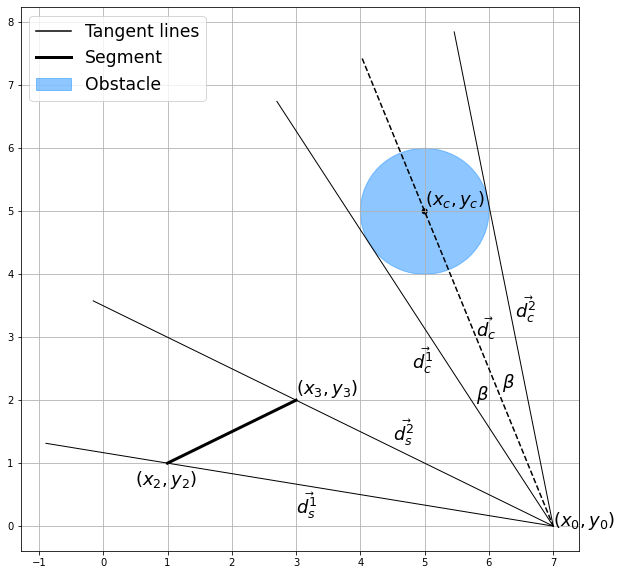
\includegraphics[width=0.48\textwidth]{final_pre_slides/root/fig_vasenkov/tangent-obstacles.jpg}
      \end{center}
    \end{wrapfigure}
    
    \vspace{0.75cm}
    \textbf{\large Tangent Lines for a Segment:}
    \begin{itemize}
      \item[-] $\vec{d_s^1} = (x_2 - x_0, y_2 - y_0)^T$
      \item[-] $\vec{d_s^2} = (x_3 - x_0, y_3 - y_0)^T$
    \end{itemize}
    
    \end{frame}
    
    \begin{frame}{Problem solution: Tangent Lines}
    \textbf{\large Algorithm:}
    \begin{itemize}
      \item[-] Find obstacles inside FOV
      \item[-] Find tangent lines to obstacles in FOV
      \item[-] Find boundary segments inside FOV
      \item[-] Find tangent lines to boundary segments
      \item[-] Sort all tangent lines by angle inside FOV
      \item[-] Iterate over sorted tangent lines, finding feasible gap with maximal distance and sufficient width
      \item[-] Output gap boundaries
    \end{itemize}
    \end{frame}
    
    % Methods comparison
    \begin{frame}{Methods comparison}
    \begin{tabular}{ |c|c| }
    \hline
     & Splitting Vectors \\
    \hline
        Advantages & Easy to extend for different obstacles \\ 
                   & Simpler implementation                 \\
    \hline
        Disadvantages & Complexity $O(KN), K \sim 10^3$     \\
                      & Can miss small objects \\
    \hline
    \end{tabular}
    
    \vspace{1cm}
    \begin{tabular}{ |c|c| }
    \hline
        & Tangent Lines \\
    \hline
        Advantages & Precise solution \\ 
                   & Complexity $O(N log(N))$ \\
    \hline
        Disadvantages & More complex implementation \\ 
    \hline
    \end{tabular}
    
    \vspace{1cm}
    N - total number of elements (obstacles + segments of the track)
    \end{frame}
    
    % Results
    \begin{frame}{Results}
    \begin{figure}
        \centering
        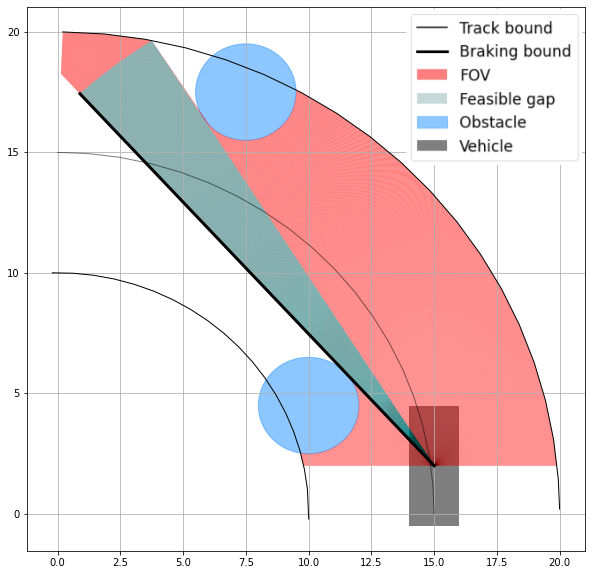
\includegraphics[width=0.48\linewidth]{final_pre_slides/root/fig_vasenkov/fov-1-labels.jpg}
        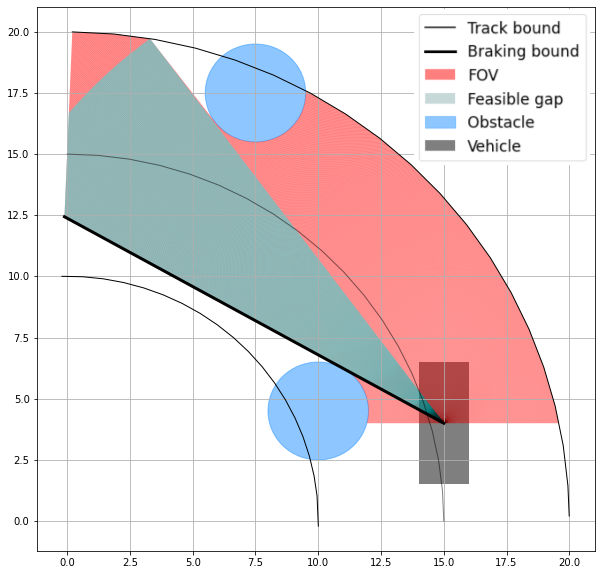
\includegraphics[width=0.48\linewidth]{final_pre_slides/root/fig_vasenkov/fov-3-labels.jpg}
        \label{fig:enter-label}
    \end{figure}
    \end{frame}
    